\subsection{Discrete-Event Trees}
In this section, advanced methods for generating discrete-event trees discussed in
\subsubsection{Stage-Decomposition with K-medoids}
Even though the algorithm presented in the previous section is able to considerably reduce the computational burden of the problem, it still takes about 15 minutes to run on a dual core machine with 2500 Mhz and 4 Gbytes RAM, using Gurobi as the MILP solver.
Using theorem \ref{thm:kmeans-kantorovich}, a heuristic algorithm can be derived, that is an order of magnitude faster than the stage-wise MILP algorithm presented above.

Consider the above MILP $\mathcal{M}_{sw}(f)$ that is solved for every father node in the tree.
This MILP is the direct solution to problem \ref{prb:DE-Kantorovich-randvar} of finding the subset of events of a discrete random variable that form the best approximation.
With the help of theorem \ref{thm:kmeans-kantorovich} we can replace the solution of the MILP with the solution to the K-medoids problem.

There are many algorithms for solving the K-medoids problem.
For the purposes of this paper, a MATLAB implementation of the standard algorithm, ``Partitioning aroud Medoids''(PAM) was used \cite{Kaufman1987}.
PAM can be viewed as an implementation of algorithm \ref{alg:kmeans}, with a more specific maximization step. The details are not the concern here. The main point is that it can be computed orders of magnitude faster than the solution to the MILP and 

The adapted algorithm is presented as algorithm \ref{alg:stagewise-kmedoids}.
It follows along the same lines as the stage-wise MILP algorithm and uses the same sets $F$ and $S_k$.
The general evolution of the algorithm follows the one depicted in figure \ref{fig:swmilp-explanation}.
\begin{algorithm}
  \KwIn{Set $I$ of $T$-stage scenarios $\xi_i^t$, tree structure $\mathcal{T}$}
  \KwOut{Scenario tree consisting of nodes $\nu_n$ and probobilities $q_j$}
  $F \leftarrow \{1\}$\tcc*{init set of father nodes with root node}
  $S_1 \leftarrow I$\tcc*{All scenarios share the root node}
  \While{$F\neq \emptyset$}{
    \ForEach{$f\in F$}{
      $F \leftarrow F\setminus \{f\}$\tcc*{remove this node from father set}
      $[m,r] \leftarrow \operatorname{PAM}(K=n_c, X=\{\xi_i^t|i\in S_f\})$\;
      \For{$l=1\ldots n_c$}{
        $k \leftarrow child(f,l)$\tcc*{get child no. $l$ of node $f$.} 
        $\nu_k \leftarrow m_l$\;
        $S_k \leftarrow \{i | r_{ik}=1\}$\;
        \If{$k$ has children}{
          $F \leftarrow F\cup \{k\}$\;
        }
      }
    }
  }
  $q_j\leftarrow $ optimal weights \tcc*{Using Algorithm \ref{alg:optimal-weights}}
  \caption{Stage-wise $K$-Medoids}
  \label{alg:stagewise-kmedoids}
verfuegungverfuegung\end{algorithm}
\subsubsection{Stochastic Search Solution to Large-Scale MILP}
While the stage-wise methodology is an easy way to reduce the complexity of the problem, it may lead to an oversimplification.
Figure \ref{fig:stagewise-failure} shows an example how stage-wise operating algorithms may yield arbitrarily bad tree approximations. 
\begin{figure}
  \centering
  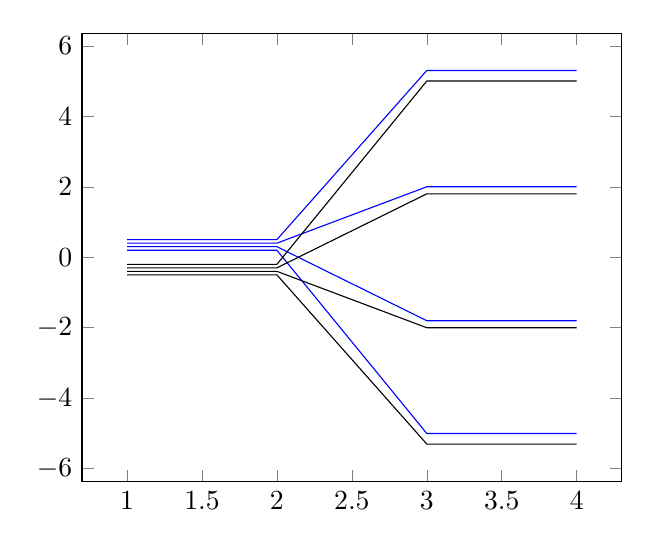
\begin{tikzpicture}
    \begin{axis}
      \addplot [color=blue] coordinates {
        (1, 0.2)
        (2, 0.2)
        (3, -5)
        (4, -5)
      };
      \addplot [color=blue] coordinates {
        (1, 0.3)
        (2, 0.3)
        (3, -1.8)
        (4, -1.8)
      };
      \addplot [color=blue] coordinates {
        (1, 0.4)
        (2, 0.4)
        (3, 2)
        (4, 2)
      };
      \addplot [color=blue] coordinates {
        (1, 0.5)
        (2, 0.5)
        (3, 5.3)
        (4, 5.3)
      };
      \addplot [color=black] coordinates {
        (1, -0.2)
        (2, -0.2)
        (3, 5)
        (4, 5)
      };
      \addplot [color=black] coordinates {
        (1, -0.3)
        (2, -0.3)
        (3, 1.8)
        (4, 1.8)
      };
      \addplot [color=black] coordinates {
        (1, -0.4)
        (2, -0.4)
        (3, -2)
        (4, -2)
      };
      \addplot [color=black] coordinates {
        (1, -0.5)
        (2, -0.5)
        (3, -5.3)
        (4, -5.3)
      };
    \end{axis}
  \end{tikzpicture}
  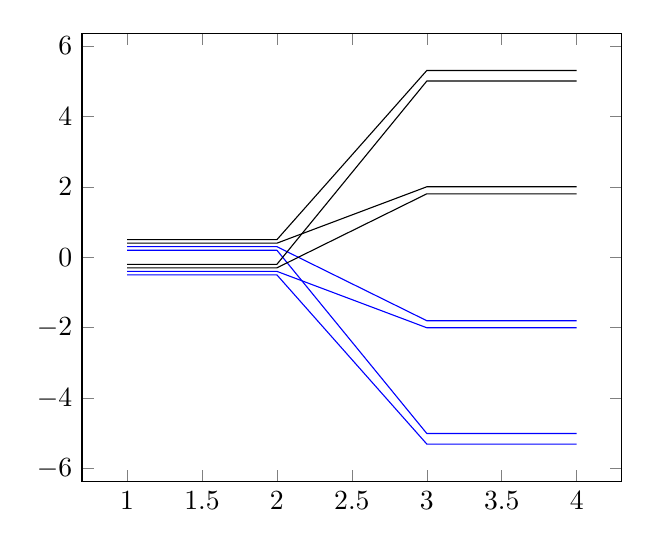
\begin{tikzpicture}
    \begin{axis}
      \addplot [color=blue] coordinates {
        (1, 0.2)
        (2, 0.2)
        (3, -5)
        (4, -5)
      };
      \addplot [color=blue] coordinates {
        (1, 0.3)
        (2, 0.3)
        (3, -1.8)
        (4, -1.8)
      };
      \addplot [color=black] coordinates {
        (1, 0.4)
        (2, 0.4)
        (3, 2)
        (4, 2)
      };
      \addplot [color=black] coordinates {
        (1, 0.5)
        (2, 0.5)
        (3, 5.3)
        (4, 5.3)
      };
      \addplot [color=black] coordinates {
        (1, -0.2)
        (2, -0.2)
        (3, 5)
        (4, 5)
      };
      \addplot [color=black] coordinates {
        (1, -0.3)
        (2, -0.3)
        (3, 1.8)
        (4, 1.8)
      };
      \addplot [color=blue] coordinates {
        (1, -0.4)
        (2, -0.4)
        (3, -2)
        (4, -2)
      };
      \addplot [color=blue] coordinates {
        (1, -0.5)
        (2, -0.5)
        (3, -5.3)
        (4, -5.3)
      };
    \end{axis}
  \end{tikzpicture}
  \caption{A stochastic process, for which algorithms that operate stagewise may yield arbitrarily bad results.
    The first plot shows the partition found by an algorithm which fixes the first stage before considering the second. 
    This yields a tree that is by far inferior to the one obtained by adjusting the tree to all stages at the same time}
  \label{fig:stagewise-failure}
\end{figure}
The MILP model for the full tree is, however, not computationally tractable.
In this section, we will present an algorithm based on genetic optimization techniques. 

When considering the full stochastic process at once, it is convenient to regard the scenarios as multidimensional events of a random variable. 
Recall from theorem \ref{thm:optimal-weights} that if the values of the nodes of the stochastic process are fixed, the Kantorovich distance o
\todo[inline]{Describe the stochastic search solution}
\todo[inline]{Create an algorithm object for the stochastic search solution}
\subsubsection{Results}
In this section, we will evaluate the scenario trees generated with the algorithms of the previous sections.
As discussed above, the approach discussed in this part is particularly suitable to problems with a discrete set of outcomes at each stage.
Therefore, we will focus on processes with that characteristic feature.
%
\paragraph{Implementations}
As all methods presented in this paper are new, the focus clearly lies on the derivation of the algorithms.
The results presented in this sections are based on ad-hoc implementations of these algorithms in MATLAB.
The MILP subproblems were solved using the commercial solver GUROBI.
The numbers on timing should be regarded only for a general orientation, and should not be judged on an absolute scale.
Many of the subalgorithms of the methods are of a heuristic or combinatorial nature.
Their performance is therefore susceptible to fine tuning, which was not conducted for the implementations.
Future implementations may therefore realize significant speedups through a better implementation of the same methods.
%
\paragraph{Testing methodology} 
Comparing scenario trees generated with different methods is not trivial.
The procedure we used to ensure relative reproducability of the results is as follows.
A set of scenarios was sampled from the original stochastic process.
This same set of scenarios was handed to each of the algorithms as input for the tree generation.
Using the same set of scenarios as input is important to not judge one of the tree generating algorithms for a singular event in its data scenarios.
The trees were then tested against ten new randomly generated sets of scenarios.
% The commercial solver Gurobi was employed to solve the MILP subproblems at each stage.
\paragraph{Coin Toss} Consider the stochastic process created by successive random coin tosses.
In order to analyze how well the algorithm does on unknown problems, we will pretend that the only information we have is a black box process that generates one scenario, which is a sequence of 3 successive coin tosses.
We, of course, know that the actual probabilities of each state.
We will compare the resulting scenario tree with
\paragraph{Log-normal SP}
\begin{figure}
  \begin{tikzpicture}
    \begin{axis} % time over number of scenarios 
      \addplot [color=black] coordinates {
        (500, 0.082675)
        (1000, 0.196757)
        (5000, 5.069326)
        (10000, 24.863489)
      };
    \end{axis}
    \end{tikzpicture}
    \begin{tikzpicture}
    \begin{axis} % 
      \addplot+[error bars/y dir=both, error bars/y explicit] coordinates {
        (500,  0.111438319659227) +- (0,0.003856365366939)
        (1000, 0.106969745621786) +- (0,0.001648309731920)
        (5000, 0.103710603975520) +- (0,0.000749656195408)
        (10000,0.103426137163199) +- (0,0.000595482018280)
      };
    \end{axis}
  \end{tikzpicture}
\caption{Results for Lognormal Distribution trees computed }
\end{figure}  
\begin{itemize}
\item the true solution, to assess the degree of suboptimality
\item with a naive tree generated by random selection of nodes from the set of scenarios. This helps us evaluate whether the extra effort put in to solve the MILP actually improved the prediction of the state.
\end{itemize}

%%% Local Variables: 
%%% mode: latex
%%% TeX-master: "da"
%%% End: 
